\documentclass[11pt,letterpaper]{article}

% Load some basic packages that are useful to have
% and that should be part of any LaTeX installation.
%
% be able to include figures
\usepackage{graphicx}
% get nice colors
\usepackage{xcolor}

% change default font to Palatino (looks nicer!)
\usepackage{apjfonts}
% load some useful math symbols/fonts
\usepackage{latexsym,amsfonts,amsmath,amssymb}

% comfort package to easily set margins
\usepackage[top=1in, bottom=1in, left=1in, right=1in]{geometry}

% control some spacings
%
% spacing after a paragraph
\setlength{\parskip}{.15cm}
% indentation at the top of a new paragraph
\setlength{\parindent}{0.0cm}


\begin{document}

\begin{center}
\Large
{\bf Ay190 -- Worksheet 10} \\
\large
Xiangcheng Ma \\
Date: \today
\end{center}

\section*{Boundary Value Problem}
(1) Using the forward Euler intergrator, I select grids of 10 points, 100 points and 1000 points and plot the results in Figure~\ref{fig1}. As the number of grid points increases, the result becomes more and more accurate.

I didn't implement a RK integrator because the structure of the current code is not comfortable to me. It would be much easier if I write the code completely by myself. To save time, I just give up this part.

\begin{figure}[th]
\centering
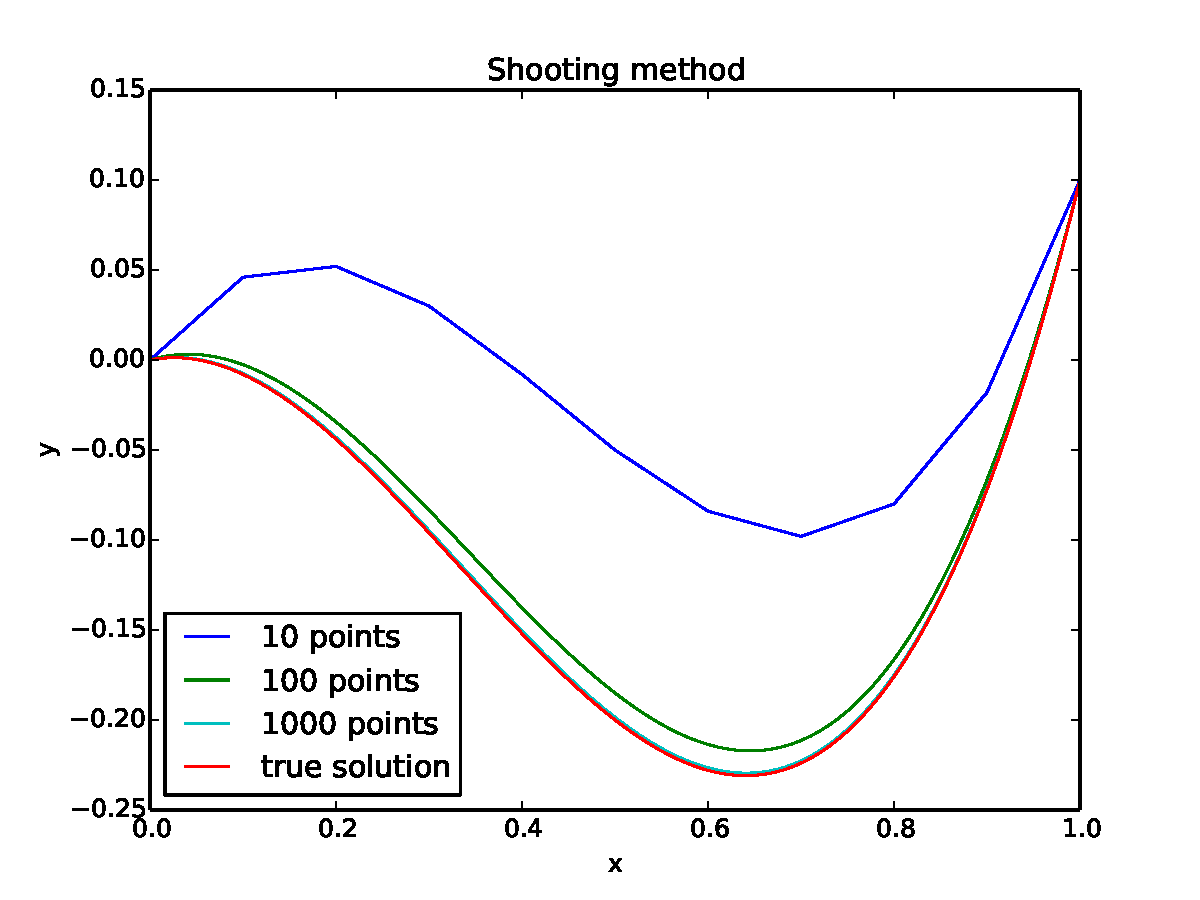
\includegraphics[width=0.9\textwidth]{fig1.pdf}
\caption{Shooting Method}
\label{fig1}
\end{figure}

(2) I write a routine {\tt finite.py} to do the finite difference method. So far this routine is limited to 1-dimensional problem with uniform grid. I take number of grid points as 6 and 10 and plot the result in Figure~\ref{fig2}.

\begin{figure}[th]
\centering
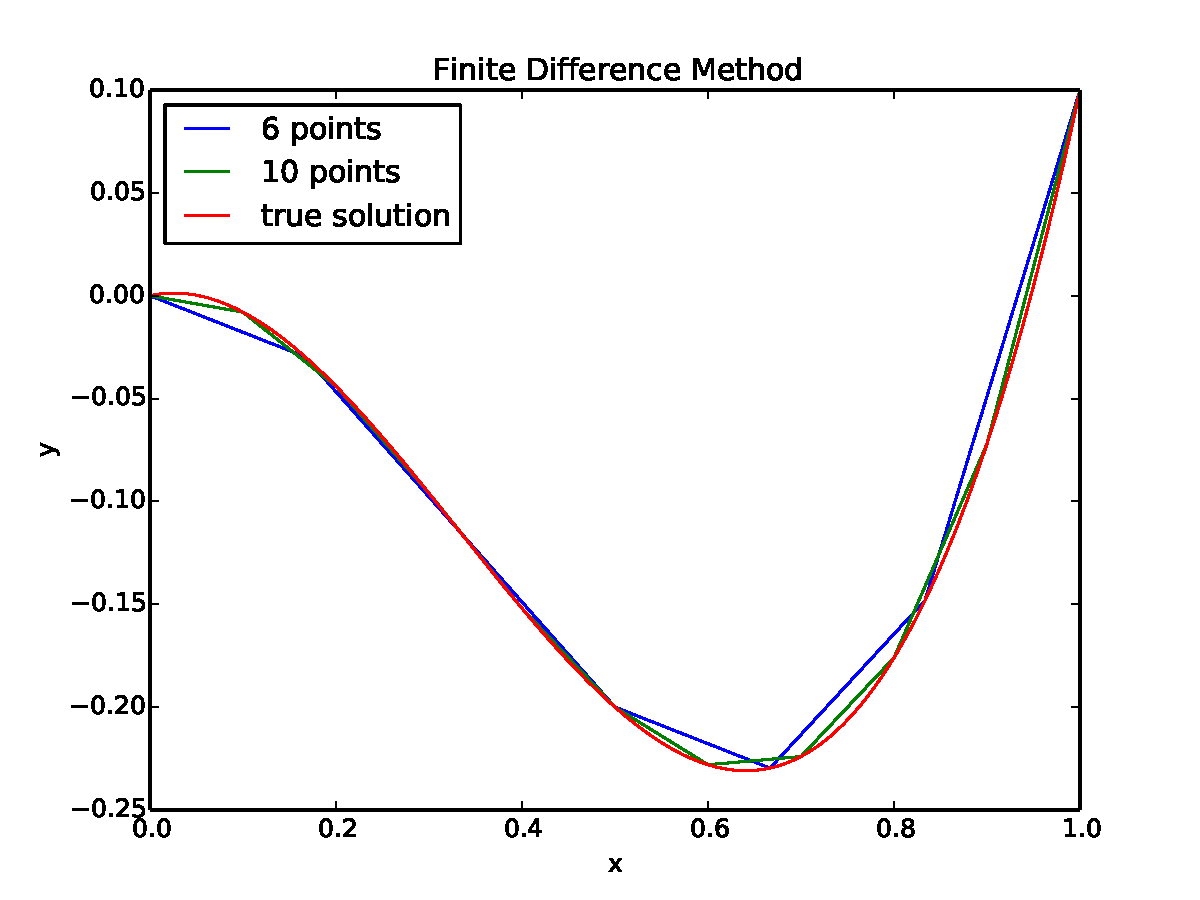
\includegraphics[width=0.9\textwidth]{fig2.pdf}
\caption{Finite Difference Method}
\label{fig2}
\end{figure}



\end{document}
